\documentclass{article}

\usepackage{layouts}

\usepackage[utf8]{inputenc}
\usepackage[T1]{fontenc}
\usepackage{mathptmx}
\usepackage{amsmath}
\usepackage{graphicx}
\newcommand{\minus}{\scalebox{0.75}[1.0]{$-$}}
\usepackage{fancyhdr}
\usepackage{url}
\usepackage{xcolor}
\usepackage{hyperref}
\usepackage{csquotes}
%\usepackage{geometry}
\usepackage{emptypage}
\usepackage[parfill]{parskip} % removes indentation of sectioning.

% For tikz images
\usepackage{filecontents}
\usepackage{tikz}
\usepackage{graphicx}
\usepackage{caption}
\usepackage{subcaption}
\usepackage{amsmath}

\usetikzlibrary{arrows}
\usepackage{pgfplots}
\usetikzlibrary{calc,fadings,decorations.pathreplacing}

\usetikzlibrary{matrix,positioning,fit,backgrounds,intersections, fit, arrows.meta, shapes}

\usepackage{titlesec}

\setcounter{secnumdepth}{4} % gives numbers to subsubsections
\usepackage{hyperref}
\usepackage{graphicx}
\usepackage{multirow}
\usepackage[margin=0.9in]{geometry}
\usepackage[acronym, nonumberlist]{glossaries}
\makeglossaries
 
\usepackage[labelfont=bf]{caption} % Gives bold figure X. 
 
\usepackage{amsmath}

\usepackage[utf8]{inputenc}

\title{Machine Learning part of theoretical background}
\author{Hanna Svennevik}
\date{February 2020}

\begin{document}
\maketitle
In this section the computational methods used for generating the numerical experiments conducted in this thesis is introduced. Starting with a short introduction to artificial intelligence. A brief introduction to the biological mechanisms the algorithms in this thesis draw inspiration from will be given. 
% Its subcategories and the biological mechanisms  relevant for the algorithms used in this thesis. 
This helps to gain insight to possible applications of different structures. 
%Presenting the autoregressive model and convolutional long short-term memory. The performance metrics used to evaluate their performance and finishing of with automatic optimization routines.
% based on bio-inspired mechanisms are introduced

The task of forecasting in time and space requires two types of intelligence. One is computer vision, to understand the spatial relation and use the underlying physical properties. The other is sequential modelling to understand the temporal evolution. Two approaches will be explored, autoregressive models (AR) and Convolutional LSTM (ConvLSTM). The AR model describes a time varying process, depending linearly on it previous values. Another method used is the ConvLSTM. Varying in space and time, capable of finding non-linear relation in the inputs.

The continuously increased popularity of deep learning can be partly explained by flexibility of the structures making it applicable for wide range of application, across many domains. All algorithms discussed is simply a mathematical framework for learning model representations in data. \textit{According to the philosophy underlying deep learning approach, if we have a reasonable end-to-end model and a sufficient data for training it, we are close to solving the problem}. (Shi et. al., 2015). 
%To the authors knowledge few/ none studies have attempted to parameterise clouds using the machine learning approach before. 

% Feed forward describes the rule of signal processing trough the network. 

\section{Artificial intelligence}
Artificial intelligence (AI) emerged from biological inspired computing. Many of the networks architectures draw inspiration from the human brain. The results of using AI is not the same as modelled as a brain, but provide a explanation to the similar jargon in AI and neuroscience. A network architecture is the designed structure. Available building blocks are neurons (nodes, units), weights (connections between neurons), rules of signal propagation, activation function (transfer function) and learning algorithms (training algorithms). For future reference, layer is a set of nodes that is not connected. Nodes in consecutive layers are connected with weights. \textbf{cite \href{https://www.sciencedirect.com/topics/engineering/neural-network-architecture}{\textbf{https://www.sciencedirect.com/topics/engineering/neural-network-architecture}}}

% For mye om receptive field.
Image recognition and sequence modelling draw parallels to human vision and memory respectively. Sequence modelling requires information about earlier stages. Storing this in memory. More advanced architectures divide it into short and long-term memory. This draws inspiration from how the memories are stored in the human brain. 

The visual cortex is the center of the brain responsible for interpreting the visual world. The receptive field of a neuron is the part of a world that activates the particular centre of the brain. \textbf{cite O'Reiley} In layman's terms, the receptive field, is the part of the image that the computer see. Receptive fields can overlap and together they assemble larger structures, like whole visual fields. Finishing each others sentences is a trivial task for humans. The reader might not be to surprised by the ending of the following sentences \textit{the clouds are in the ... sky.} \textbf{cite some blogpost?} \textbf{or :}  The reader might not be to surprised that the by the following \textit{the clouds are in the ... sky.}

% Inspird by Chollet book
In encounters with geoscientists the author often get the question: \textit{Whats \textcolor{red}{"What is" eller "what's"} the difference between machine learning and artificial intelligence?} They are not different fields, but machine learning (ML) is a subfield \textcolor{red}{"is a subfield" eller "are subfields"?} of AI. In fact, its \textcolor{red}{"it is" eller "it's"} worth mentioning that there is a subfield of ML known as deep learning (DL). See graph in Figure \ref{fig:subcategories_AI}, deep learning is a subfield of machine learning, making it a subfield of artificial intelligence. %Deep learning provide a improved.
The origin of the subfields have a historical explanation. They are all linked to significant advances, they will be explained drawing parallels to computer chess. 
\begin{figure}
    \centering
     
    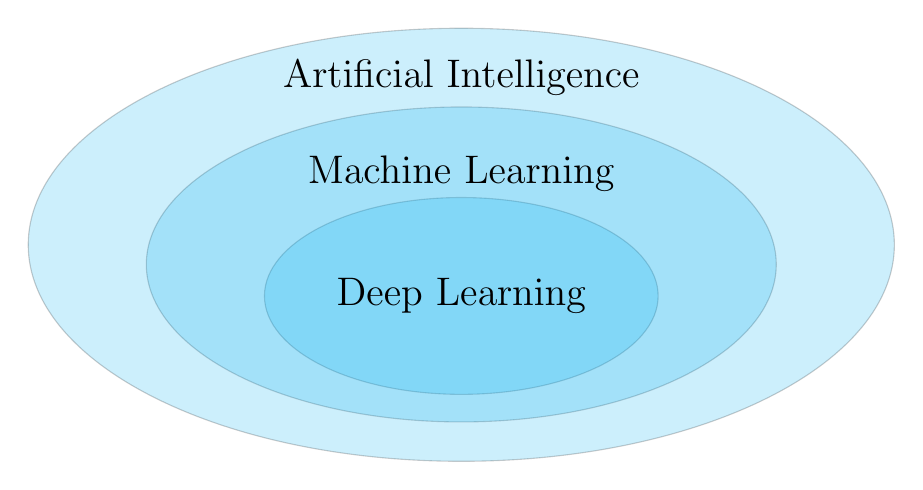
\begin{tikzpicture}
        \draw [black, fill=cyan, opacity = 0.2]  (2, -0.65) ellipse (2.5 and 1.25); % DL 
        \draw [black, fill=cyan, opacity = 0.2]  (2, -0.25) ellipse (4 and 2); % ML
        \draw [black, fill=cyan, opacity = 0.2]  (2, 0) ellipse (5.5 and 2.75);     % AI
        \node at ($(2, 2.125)$) {\Large Artificial Intelligence}; % +(2 and -0.65)
        \node at ($(2, 0.9)$) {\Large Machine Learning};
        \node at ($(2, -0.65)$) {\Large Deep Learning};

    \end{tikzpicture}
    
    \caption{Graph illustrating the subfields of AI. ML is a subfield of AI, DL is again a subfield of ML. The sketch is inspired by figure 1.1 in \textbf{Chollet book cite properly}.}
    \label{fig:subcategories_AI}
\end{figure}
AI  dates back to the fifties. Pioneers was debating if it was possible to \textit{automatise \textcolor{red}{usikker på om det er best å bruke "automatise" eller "automatize"} task normally performed by humans}. Three factors determining the advances of the field; data, hardware and algorithms. \textbf{cite Chollet book} This explains why there often is a significant time gap between the idea and breakthroughs of architectures. Convolutional neural networks (CNN) being developed in the eighties, lying dormatory until 2012, when AlexNet (a CNN architecture) wins Image net competition, a image recognition contest. \textbf{cite something} Long short term memory was invented in 1997. Breakthough in X. 

AI started by automating tasks normally performed by humans. Computer chess is the longest studied problem in the history of artificial intelligence. The evolution of chess provides good examples on the evolution of AI.
In 1951 Alan Turing was the first to publish a program, on paper, capable of playing a entire game of chess.
Starting with explicitly trained programs. This falls in the category of AI and not ML. \textit{Learning, in the context of ML, describes the automatic search for a better representations.} ML strives to go beyond what we know. This kind of computer chess is fed with many examples of played chess game, frame for frame. Given data and the answers, the goal of ML is to deduct the rules (a program). \textbf{cite something}

The network is presented with many examples and is trained rather than explicitly programmed. Geoscientists may be more familiar with the phrasing calibrating when it comes to statistical models, which essentially is the same thing.

Deep in the context of \textit{deep learning} relates to the number of layers contributing to a network. DL expands the ideas from ML using deeper network, e.g. more layers. A layer is a set of nodes. The connections between the layers are the trained units, also known as weights. After the invention of deep learning, traditional machine learning is sometimes referred to as shallow learning. Linear regression (LR) is ML algorithm predating computers which is still useful today. Traditional LR can be derived using shallow learning methods.

The frontier of chess playing programs is AlphaZero. The deep reinforecent architecture trained using self-play, without any previous knowledge of rules. 
%ML is often referred to as shallow learning since its concerned  \textcolor{kan du droppe "its concerned"? og heller skrive " ML is often referred to as shallow learning since its training structure consist of one or two layers"?} with training structures with one or two layers. 

% Explain glossaries or words that are used a lot.
Intelligence, in the context of artificial intelligence is still a topic of debate. Traditionally a machine would be considered intelligent if it would beat a human at a given task. Etter at DeepBlue slo Gary Karsparov i 1997 gikk det opp for forskere at de hadde lært lite og ingenting om human cognitive system by solving this task. Det ble tydelig at de egenskapene mennesker må sitte inn med for å løse et slik problem er elt anderledes enn de maskiner må sitte inne med. This has later been abandoned. \textbf{chollet google artikkel}

There are lot of different types of machine learning, suitable for solving different tasks. Figure \ref{fig:machine_learning_categories} shows the types of ML and their subcategories. \textbf{Kan man si at de finnes for deep learning, men siden det er mer generelt en som så velge jeg og snakke om dem som underkatergorier av machine learning.}

Many of these subcategories also exist for DL, simply by adding the prefix 'deep'. \textcolor{red}{(Nytt avsnitt?)}Supervised learning is the part of machine learning concerned with learning the relation between input data, x and labelled data, y. Regression predict continuous values. Replicating a function. Classification is discrete, since it assigns a category to the input. 

Reinforcement learning is a goal-oriented algorithms, most known for playing chess, solving labyrinths and lately \textcolor{red}{for?} active flow control \textbf{Cite Jean Rau, three papers}. \textcolor{red}{(Nytt avsnitt?)} 

Unsupervised learning tries to detect patterns in unlabelled data. This includes clustering and dimensionality reduction. Dimensionality reduction has been used by climatologist for decades in order to remove seasonal variation \textbf{cite Benestad}. Unsupervised and reinforcement learning is out of the scope of this thesis and will not be discussed further.
\input{graph.tex} 
\textcolor{red}{Kan du sette det opp mer oversiktilig? Eller blir det for simpelt?}
\begin{itemize}
    \item \textbf{Supervised learning}: part of machine learning concerned with learning the relation between input data, x and labelled data, y.
    \begin{itemize}
        \item Regression\\predict continuous values. Replicating a function.
        \item Classification\\discrete, since it assigns a category to the input.
    \end{itemize}
    \item Reinforcement learning
\end{itemize}

\textcolor{red}{Nå har du en ny figur med underkategorier i ML, men du har tidligere skrevet at DL er en del av ML, så ville i så fall skrevet i figurteksten at kategoriene også er overførebare til DL eller hvordan sammenhnegen med at DL er under ML, men så har ML kategorene du beskriver i figur 2, mens DL er det en del av noen kategoriene, men ikke alle. Prøv gjerne å beskriv eller finn figur som beskriver dette }
\textcolor{red}{ser at input i de neste figurene er blå, kanskje du kan velge en annen farge på figur 1 og figur 2. Hva med oransje? Veldig fint at du har ulike fargenyanser på figur 1 for de ulike delfeltene.}

\subsection{Autoregressive models} \label{sec:ARmodels}
The autoregressive model (AR) is a form of linear model where values from previous time steps are included as predictor variables. 
\begin{equation} \label{eq:AR_traditional}
    \hat{Y}_n = \hat{\beta}_0 + \sum_{i = 1}^{N} Y_{n-i} \hat{\beta}_{i}
\end{equation}
Equation \eqref{eq:AR_traditional} describes how to make a prediction based on the optimal weighs, $\beta_i$. $n$ denotes a particular time step, while $N$ denotes the order of the model, also known as number of previous time steps. $\beta_0$ is the bias. $i$ is a counter going backward in time.
\begin{equation} \label{eq:AR_expression}
    \hat{Y}_n = \hat{\beta}_0 + \sum_{j=1}^p X_j\hat{\beta}_j + \sum_{i = 1}^{N} Y_{n-i}\hat{\beta}_{i}
\end{equation}
Expanding the traditional AR model to include other predictors, $X$ yields the expression in Equation \ref{eq:AR_expression}. $p$ denotes the number of predictors. The other symbols are described above referring to Equation \ref{eq:AR_traditional}.
\begin{equation} \label{eq:AR_solution}
    \hat{ \beta } = \left( \textbf{X}^{*^T}\textbf{X}^* \right)^{-1}\textbf{X}^*\bar{y}
\end{equation}
Let $X^*$ be the concatenation of X and Y. In mathematical terms, $X^*=[X, Y]$. Using mean squared error loss, there exist an analytical solution to the optimization problem. 


The expression for finding the optimal solution, $\beta_0,...\beta_i$, in a matrix form is given in Equation \eqref{eq:AR_solution}. The optimal solution is the best solution based on the training data available. The analytical solution is computationally very fast, as long as the matrix $X^*^TX^*$ is non-singular and thus its inverse exits.

\section{Artificial Neural Networks} \label{sec:artificial neural networks}
\input{one_layer_mlp}
Artificial neural networks (ANN) are composed of artificial neurons and weights. Figure \ref{fig:one_layer_mlp} illustrates nodes as circles and weights as arrows. It is a example of a 2-layer ANN. The nodes are structured in layers. The input layer containing four input nodes, the hidden layer, five nodes and the output layer, three nodes. The dimensions of the input and output layers are determined by the task at hand. The number of hidden layers and the number of nodes are tunable parameters, called hyperparameteres. Neurons of one layer is only connected to the immediately preceding and following layers. Weights are the connections between nodes in neighbouring layers. All networks have input, output and zero or more hidden layers. Large networks of these simple neurons are able to perform complex calculations. 
\input{activation_mlp}
Figure \ref{fig:activation_one_node} shows the computation which takes place in a node in the hidden layer, a green dot in Figure \ref{fig:one_layer_mlp} The sum of the weighted input and bias are sent trough the activation function, g. 
\begin{equation} \label{eq:ANN_forward_pass}
    y = g(\sum_{i=1}^n w_{L, i} x_i + b_L)
\end{equation}
The activation in a arbitrary layer, L is given by Equation \eqref{eq:ANN_forward_pass}, where $b_L$ is the bias and $w_L$ is the weights matrix and $n$ is the number of input nodes. The weighted activation is then passed to the output nodes, the red dots. 

\subsection{Convolutional neural networks} \label{sec:convolutional neural network}
Computer vision is a field of artificial intelligence concerned with interpreting the visual world. One popular structure for visual tasks are the convolutional neural network. %Its said to resemble the visual cortex, the centre in the brain which processes the visual information. 
Computer see images as a grid of numbers. Often decoded in red, green and blue (RGB) channels. Each of each of the grid cells, also called pixels, contain the signal from the color decoded into numbers ranging from 0 to 255. The machine needs to learn how to extract the necessary information about these pixels to perform a task. More layers increases the models ability to extract these complex structures. Resulting in an improved model performance. 
\input{convolution}
A convolution is a mathematical operation. The sum over element wise multiplication. This is illustrated in Figure \ref{fig:convolution}. The filter is green, this is placed over the filled blue section, producing the red output pixel. The entire red grid is called a feature map. The blue grid is the input, and as you can see only parts of the image (the filled) blue section contributes to the activation. \textit{Receptive field} is known as the pixels contributing to the activation in a pixel (i.e. the value). For instance the receptive field of the filled red pixel is the filled blue submatrix.

%\textcolor{red}{Generelt : Ufullstendige setninger. Ønsker mer forklaringer av hva convolution er. Synes forklaringen med grid celler med tall fra 0 255 var bra. Gir mening for folk. Og at flere lag gir bedre forståelse av bildet. Veldig bra! Men la dette få komme frem. }

\input{convolution_connection_between_layers}
Convolving a filter over the input image generates a feature map. If it happens to be the last layer, it is common to refer to the results as the output instead. Even though there is no differences. Figure \ref{fig:convolution_padding} shows a 2D-convolution with filter of size $3\times 3$. Filters are often square (not a strict requirement) and the height, $f_h$ and $f_w$ are odd numbers (not a strict requirement either). The origin is the position of the kernel which is above the current output pixels. The connections between the layers are intended to illustrate the part contributing to the pixel as well as highlighting the receptive field. With the purpose of including the signal from the boundary and or preserving the input shape. The gray shaded area is the padded. 
\input{2_layer_convolutional}
Working with RGB-images requires 3D-convolution. As mentioned earlier, neural networks are a stack of layers. The output from the previous layer becomes the input to the next layer. To be clear, feature maps, activations and outputs are the same thing. It is the result of convolving the input. The activations are computed based on a input volume, including information across channels. Meaning it knows about all the colors of a RGB-image. Figure \ref{fig:conv_layers} shows a two layer convolutional neural network trained on RGB-images. The input layer is a RGB-image. The first convolutional layer has seven channels (feature maps), these are produced by seven filters. Filters are trained to extract useful features. The second convolutional layer is produced by five filters, all convolving layer 1. It worth noting it is this shallow for illustrative purposes. Networks are usually a lot deeper. Given raw input (i.e. normalized images), the first layers detects low level features like edges, corners and circles. The last layers assemble the features to more complex structures like houses or dogs. The dashed volumes represent the receptive field for differeent pixels, illustrated as circles. Since each of the layers depend on the previous one, the receptive field of the output node \textbf{give it a name} depends on a large portion of the input image.

\textbf{Bruke som bilde text ..?} Each convolutional layer contains multiple filters, thus producing stack of feature maps. The trailing layer get this stack as input, producing activations based on all channels. For each layer it contains representations of the structures found in the previous layer. The filters are the weights trained to find useful structures. In each convolutional layer multiple of these filters are passed over the image. Small filters allow you to focus on small features in the data. Larger filters allows you to find coarser relations. 

Unlike fully connected layers, the nodes in the first layer \textcolor{red}{The input layer? (ref fig. 3)} are not connected to all the input nodes \textcolor{red}{Så ikke som i figur 3?}. The filters are square, and contains the parameters learned using convolution. This allows you to look for the same structure all of the image. %Reduces the number of trainable parameters and making it more robust against overfitting.

\subsection{Recurrent Nets} \label{sec:reccurent_nets}
% Recurrent betyr tilbakevendende
% Sequential modelling has had a great success in applications such as machine translation and speech recognition 
Recurrent neural network (RNN) is a class of artificial neural networks. Developed for studying patterns in sequential data such as time series, audio or text. Figure \ref{fig:rnn} shows the structure of a simple RNN. In simple terms RNN receives a input, produces an output and passes it back to itself. 

In Figure \ref{fig:rnn}, A denotes a recurrent unit, $x_t$ denotes the input data and  $h_t$ denotes the hidden state. The output from an arbitrary node, $i$ is $h_i$. The loop explains the origin of the name recurrent neural network. The output at each time step is dependant on the previous inputs. $h_0$ is only dependant on $x_0$, while $h_t$ is dependant on $x_0, x_1, \cdots, x_t $. A RNN uses the same weights on the input and hidden states for all time steps. \textbf{forrige setning er forvirrende}. Here t denotes the length of the training sequence.
\input{rnn}
The "memory" stores the useful information from $x_0, x_1, \cdots, x_t $ needed to make a prediction. Performing the same task on all inputs along the sequence. This reduces the complexity of parameters and in turn reducing the risk of overfitting. Obtaining a more general relation between \textbf{input and output..?}
\input{rnn_unrolled}
Figure \ref{fig:rnn_unrolled} shows the recurrent network unrolled in time. The way of structuring it resembles the earlier structures discussed in Section \ref{sec:artificial neural networks}. The connection between the nodes %in this kind of networks 
are a directed graph along a temporal sequence. The output from the previous step is fed into the next. 
% It is used to predict the next word in a sentence or the next tone in a song.  
%%%%%%%%%%%%%%%%%%%%%%%%%%%%%%%%%%%%%%%%%%%%%%%%%%%%%%%%%%%%%%%%%%%%%%%%%%%%%%%%%%%%%
Learning long term dependencies can be a challenging. Learning is done by backpropagating the error signal thought the network. For more details see Section \ref{sec:backprop_learning_algorithm}. Working with longer sequences the error signal tend to blow up or vanish. Exploding gradients can cause the weights to oscillate. Learning from small or vanishing gradients takes ages, or might not learn anything at all. More advanced forms of recurrent nets control the information flow using gates. \textbf{cite 1997 and cite 1999 learning to forget.}

\subsubsection{Long Short-term memory network, LSTM} \label{sec:lstm}
%\textbf{Use recurrent self-connections instead of loops} \textcolor{red}{Ufullstendig setning}. 
The memory unit introduced by Sepp Hochreiter and Jürgen Schmidhuber in 1997 set performance records in multiple domains. The paper introduces gates to regulate the flow of information. A gate is structure that can be opened or closed. Having values in the range zero to one, it truncate the noise signal from the input and the output. They propose an approach for constant error flow in order to alleviate the issues with exploding or vanishing gradients. The original memory cell contains input and output gates. Gers et. al. 1999 proposed to add an additional gate, the forget gate. The idea was to enable the LSTM to reset its own memory. Resetting the memory releases internal resources and enable you to learn even more.

Because of the interdisciplinary nature of this thesis this section provides a comprehensive walk through the LSTM cell and its relevant equations. The memory unit is displayed in Figure \ref{fig:lstm_unit}. The legend describing the different components of the computational graph is available in Figure \ref{fig:legend_lstm}. The information flow thought the cell is regulated by three gates; the forget gate, the input gate and the output gate. These gates are neural networks. The forget gate learn what part of the cell state (the long-term memory) it should forget. The input gate learns the information from the input it should add to the cell state. The output gate learn which information it should send to the output. The process of training is repeated until the network reaches an acceptable performance. In other words \textit{the extent to which this potential can be exploited is limited to the effectiveness of the training procedure applied}. 
% Attempt to explain the figures.
\textit{For each training instance,  the algorithm }
There is two types of techniques involved in the training procedure, forward- and backward pass. A forward pass 
propagating the input trough the network. This is also what you do, when you make a prediction \textcolor{red}{eksempel?}. In the process of adjusting the weights to find the optimal solution you use backpropagate the error signal \textcolor{red}{You backpropaget the error signal?}. More details concerning gradient based learning in Section \ref{sec:backprop_learning_algorithm}.

% Introducing some terminology, a prediction is the result of forward passing the information through the network. 

\subsubsection{Feed forward} \label{sec:forward_pass_lstm}
\begin{figure*}[hp]
        \centering
        \begin{subfigure}[b]{0.475\textwidth}
            \centering
            \input{lstm.tikz}
            \caption[Channel WV 6.2]
            {{\small Recurrent unit. LSTM cell.}}
                %\\ \\ \color{white}{ooooooooooooooooooooooooo} 
                
            \label{fig:lstm_unit}
        \end{subfigure}
        \hfill
        \begin{subfigure}[b]{0.475\textwidth}  
            \centering 
            \input{1cell_state_core_idea.tikz}
            \caption[]%
            {{\small The cell state. Keeping track of the long term dependencies.}}    
            \label{fig:cell_state_information_flow}
        \end{subfigure}
        \vskip\baselineskip
        \begin{subfigure}[b]{0.475\textwidth}   
            \centering 
            \input{3_forget_gate.tikz}
            \caption[something]
            {{\small   The forget gate: $f_t = \sigma \left(W_f\dot \left[h_{t-h}, x{t} \right] + b_f \right)$ 
            \\ \\ \color{white}{ooooooooooooooooooooooooo} }}

            \label{fig:forget_gate}
        \end{subfigure}
        \quad
        \begin{subfigure}[b]{0.475\textwidth}   
            \centering 
            \input{4_input_gate.tikz}
            \caption[]
            {{\small Candidate information: $\Tilde{C_t} = tanh \left( W_C \dot \left[ h_{t-1}, x_t \right] + b_C \right)$  } \\ \\  The input gate: $i_t = \sigma \left( W_i \dot \left[ h_{t-1}, x_t \right] + b_i \right)$}

            \label{fig:input_gate}
        \end{subfigure}
                \begin{subfigure}[b]{0.475\textwidth}   
            \centering 
            \input{5_update_cell_state.tikz}
            \caption[something]%
            {{\small Updating the cell state, $C_t = f_t * C_{t-1} + i_t*\Tilde{C_t}$ \\ \\ \color{white}{ooooooooooooooooooooooooo}}}

            \label{fig:update_memory}
        \end{subfigure}
        \quad
        \begin{subfigure}[b]{0.475\textwidth}   
            \centering 
            \input{6_output_gate.tikz}
            \caption[]
            {{\small The output gate: $ i_t =\sigma \left( W_o \dot \left[ h_{t-1}, x_t \right] + b_o\right) $
             \\ \\ Updating the hidden state, $ h_t = o_t*tanh\left( C_t \right)$ }}

            \label{fig:output_gate}
        \end{subfigure}
        \caption[ havner dette i figurlista ]
        {\small Walk trought the components of a LSTM and the relevant equations. Inspired by \href{https://tex.stackexchange.com/questions/432312/how-do-i-draw-an-lstm-cell-in-tikz?rq=1}{https://tex.stackexchange.com/questions/432312/how-do-i-draw-an-lstm-cell-in-tikz?rq=1} }
        \label{fig:LSTM_all}
    \end{figure*}
\input{legend}

Figure \ref{fig:lstm_unit} show a computational graph of a LSTM cell. This cell i\textcolor{red}{s} special \textcolor{red}{special? Hva mener du med det?} recurrent unit. The following subplots highlights the graphs relevant for gates and necessary calculations. Like the human brain, the LSTM cell has it\textcolor{red}{s?} own memory. The LSTM has a long term memory, know\textcolor{red}{n} as the cell state and the short term memory referred to as the hidden state \textcolor{red}{
Burde komme når du introduserer figuren sammen med den neste setningen}. The hidden state is the output passed to the next cell. Figure \ref{fig:cell_state_information_flow} show\textcolor{red}{
s} the information flow of the cell state. It is affected by some linear interactions, \textcolor{red}{but?} this is very simple and the flow often remain unchanged. Structures like gates regulate the flow of information. 




The gates are neural networks layers with sigmoid \textcolor{red}{hva er det?} activation. 

The sigmoid function truncates the output from the gates to range between zero and one. For more information see Section \ref{sec:transforming_cloud_cover}. Figure \ref{fig:activation_func_plus} shows the sigmoid and tanh functions. Zero represents a closed gate, while one describes a wide-open gate. For each time step in the sequence the LSTM receives a\textcolor{red}{n} input and a \textcolor{red}{dropp "a"} the previous hidden state \textcolor{red}{
Hva mener du her?}. These \textcolor{red}{are} sent trough all gates. The gates in the LSTM network are multiple the trained neural networks \textcolor{red}{Skjønner ikke hva du mener?}. To sum up, at each time step some memories are removed and others are added. The cell state is then passed t\textcolor{red}{h}rough a tanh-function and filtered by the output gate. For a more detailed description see Sections \ref{sec:forget_gate} to \ref{sec:output_gate}. \textbf{cite colah blogpost ?}
% http://colah.github.io/posts/2015-08-Understanding-LSTMs/

\textcolor{red}{Denne seksjonen trenger litt bearbeidelse. Synes begynnelsen er tung og jeg skjønner veldig lite, men når jeg kommer nedover i teksten så blir jeg sånn " åååh, hvorfor sa du ikke det tidligere?". Her burde man kanskje prøve å tenke ut hva som er viktigst og gi det overordnede først?}

\paragraph{Forget gate} \label{sec:forget_gate}
\textcolor{red}{Ikke ha seksjoner på fjerde nivå. Det blir veldig oppstykket og man får lite flyt i teksten}
Based on the new input, the previous hidden state and the cell state\textcolor{red}{,} the forget gate determines which instances from the memory to remove. Regulating the information that stays in memory free\textcolor{red}{z?}s up space to learn new things. The gate is initialized to 1, thus it can't forget anything until it has learned to forget. Exhibiting the same behavior as the original LSTM units. Equation \eqref{eq:CLSTM2_forget_gate} shows the expression used to train the gate. This is illustrated in the computational graph shown in Figure \ref{fig:forget_gate}.

\begin{equation} \label{eq:CLSTM2_forget_gate}
        f_t = \sigma \left( W_{xf}*x_t + W_{hf}*H_{t-1} + W_{cf}\circ C_{t-1}+b_f \right) 
\end{equation}

%%%%%%%%%%%%%%%%%%%%%%%%%%%%%%%%%%%%%%%%%%%%%%%%%%%%%%%
\paragraph{Input gate}  \label{sec:input_gate}
The input gate regulates what information to store from the input. Its aim is to clean the input by reducing the noise signal \textcolor{red}{Kanskje bedre å skrive " The aim of the input gate is to ..."?}. This is done by Equations \eqref{eq:CLSTM1_input_gate} and \eqref{eq:CLSTM3_cellstate}. These computations are also shown in Figure \ref{fig:input_gate}.

\begin{equation} \label{eq:CLSTM1_input_gate}
    i_t = \sigma \left( W_{xi}*x_t + W_{hi}*H_{t-1} + W_{ci}\circ C_{t-1}+b_i \right) 
\end{equation}

\begin{equation} \label{eq:CLSTM3_cellstate}
        C_t = f_t \circ C_{t-1} +i_t\circ tanh\left( W_{xc}*X_t + W_{hc}*H_{t-1} + b_c \right)
\end{equation}

%%%%%%%%%%%%%%%%%%%%%%%%%%%%%
\paragraph{Output gate}  \label{sec:output_gate}
Purpose of this gate is to remove noise from the output. Preventing misrepresentations of the hidden state. \textbf{cite LSTM 1997} The computational graph is illustrated in Figure \ref{fig:output_gate}.
By filtered refers to the component wise multiplication with a gate \textcolor{red}{?? Skjønner ikke??}. This produce the output and hidden state. The latter one \textcolor{red}{The hidden state?} being the short term memory. Recall that sigmoid takes values in the range 0 to 1 and tangens hyperbolicus, tanh takes values between -1 and 1.

\begin{equation} \label{eq:CLSTM4_output_gate}
        o_t = \sigma \left( W_{xo}*X_t + W_{ho}*H_{t-1} + W_{co}\circ C_{t}+b_o \right)
\end{equation}

\begin{equation} \label{eq:CLSTM5_hidden_state}
        H_t = o_t \circ tanh \left( C_t \right)
\end{equation}

\subsection{Convolutional LSTM}  \label{sec:convolutional_lstm}
A variant of the LSTM network is the convolutional lstm. In this structure the gates are replaced by convolutional neural networks \textcolor{red}{Hva er convolutional neural networks?}. This allows the LSTM network to support multi-dimentional data., capturing the spatiotemporal structure in the data. 
% The updated equations.
More detail on convolutional layer can be found in Section \ref{sec:convolutional neural network}. The key equations in convolutional LSTM is listed in Equation (\ref{eq:CLSTM2_forget_gate}) - (\ref{eq:CLSTM5_hidden_state}). Here $\circ$ denoted the Hademand product, which is a component wise multiplication, and * is convolution \textcolor{red}{Dette må komme i tilknytning til lignigene og ikke så langt nede}. \textbf{Move the above equations to this section or }
\textbf{GOAL: Avoid to many duplicates of variant of the same equation. }


\subsection{Padding (and Stride?)} \label{sec:padding}
% Add equation to calculate how much zero padding is needed to make a prediction of the same size.
The convolution operation shrinks the dimensions of the feature map, according to Equation \eqref{eq:output_size}. The degree of shrinkage \textcolor{red}{shrinking?} depends on \textcolor{red}{the} filter size, padding and stride. Padding zeros along the edges has an additional benefit of including the signal from the boundaries. Stride determines how far you move the filter between convolutions. In other words it control how you convolve around the input volume. Figure \ref{fig:convolution_padding} shows a example with a zero padding of one. This is sufficient to keep the input dimension using a filter of dimensions $3 \time 3$. Which can be shown by plugging the dimensions into \eqref{eq:padding_same}.
\textcolor{red}{Er zero padding == padding zero?}

For a arbitrary image. Some definitions,
\begin{enumerate}
    \item image size, $n\times n$
    \item filter size, $f\times f$
    \item padding size, p
    \item stride, s
    \item output size, $o \times o$
\end{enumerate}

\begin{equation} \label{eq:output_size}
    o = \frac{n+2p-f}{s} + 1
\end{equation}
In some cases \textcolor{red}{it can} be \textcolor{red}{eller "it is useful"} useful to have the same shape of input and output. This is called \textit{padding same}. Solving the equation \eqref{eq:output_size} for $p$ using $o=n$ yields the following expression.
\begin{equation} \label{eq:padding_same}
    p = \frac{n\left(s-1\right)-s+f}{2}
\end{equation}

\subsection{Learning algorithm} \label{sec:backprop_learning_algorithm}
Learning is a time consuming task. The fundamental trick in deep learning is to use the performance metric as a feedback signal to adjust the weights. Its \textcolor{red}{"It adjustes..." eller "It adjust"} adjusted in the direction of the lowest loss score for the current example (i.e. the current batch). The adjustment is the job of the optimizer, which implements backpropagation algorithmn which is the central learning algoritmn. This section aims to build a understanding of backpropagation trough time without referring to any significant mathematics. If you are interested in the mathematics behind this, read X and Y. 


\textit{Learning means finding a suitable representation of model parameters that minimize a loss function for a given set of training data samples and their corresponding targets.}


\textcolor{red}{Tanker: 
- Veldig mye henvisninger til andre seksjoner (see section ....) noe som er litt slitsomt for leserne. Prøv å samle informasjon som henger sammen og legg heller til mer relevant informasjon senere. 
- Er neurons og weights det samme?
- Hva er networks? 
- Hva er convolution? 
- Hva er AR models? 
}
\section{Jonah stop, the following text is just notes on things i might write in the future. Some figures might have snuck passed this soft barrier thats all.}

Mye av seksjonene nedenfor er fordelaktig å skrive når jeg har trent netverkene. Det er hvertfall tanken 

\subsection{Raw input data and Activation function}
Representations of data is stored in the form of activation's. Common activation functions are displayed in Figure \ref{fig:activation_func_plus}

\begin{figure}
    \centering
    \includegraphics[scale = 0.5]{activation_functions_and_derivatives.png}
    \caption{Figure showing the shapes of activation function. Both sigmoid and tanh saturate at one, and vanish for 0 and -1 respectively. Gradient based learning doesn't learn the. ReLU doesn't have this problem with saturation.}
    \label{fig:activation_func_plus}
\end{figure}

\input{convolutional_layer}

\subsubsection{Transforming data} \label{sec:transforming_cloud_cover}
\textbf{Inverse of sigmoid is often refered to as logistic sigmoid?}
Transformation of data us useful for avoiding predicting unphysical values. As well as keeping digits from exploding.
A common approach for values in the range zero to one is using the inverse of the sigmoid function, shown in figure \ref{fig:activation_func_plus}. The transform uses values from the entire real axis $(-\infty, \infty)$. 
%\input{Chapter2_Theory/tikz/sigmoid.tikz}
Tranforming the data using sigmoid and then squazing it back between 0 and 1. 
Continous models can learn out-of-sample values. In this case it would be unphysical.

\subsection{Loss/ Metrics}  \label{sec:metrics}
In order to acquire a certain skill you need a measure determining how close you are. 
Use the sum of square or absolute values in order to not penalize point on the lower side of the line. Or not having to deal with negative distances. 
\begin{equation} \label{eq:mse}
    MSE(\hat{y},\hat{\tilde{y}}) = \frac{1}{n} \sum_{i=0}^{n-1}(y_i-\tilde{y}_i)^2
\end{equation} 

\begin{equation} \label{eq:ase}
    ASE(\hat{y},\hat{\tilde{y}}) =  \sum_{i=0}^{n-1}(y_i-\tilde{y}_i)^2
\end{equation} 

\begin{equation} \label{eq:r2}
    R^2(\hat{y}, \tilde{\hat{y}}) = 1 - \frac{\sum_{i=0}^{n - 1} (y_i - \tilde{y}_i)^2}{\sum_{i=0}^{n - 1} (y_i - \bar{y})^2}
\end{equation} 
where mean value of $\hat{y}$ is defined as $\bar{y} =  \frac{1}{n} \sum_{i=0}^{n - 1} y_i$. $R^2$ describes how much of the variation in the dataset you are able to capture with your model.

\subsection{Generalization} \label{sec:generalization}
% Move overfitting here
Finding a suitable curve for a set of points. Working with real data, noise is inevitable. In order to compensate, data is split into training and test (validation) sets. % better to call it something like generalization..?
Overall goal is to achieve the most general relation. \textit{For prediction purposes they can sometimes outperform fancier non-linear models, especially in situations with small numbers of training cases, low signal-to-noise ratio or sparse data.} \textbf{Hastie et al.} Overfitting becomes evident when you have a increase in the difference between the test- and training error. In non-mathematical terms, you have adjusted to much to the training data and where not able to find the general relation, program or "rules". See Figure \ref{fig:linreg_overfitting} 

\begin{figure}[hp]
    \centering
    \includegraphics[scale = 0.5]{generalization.png}
    \caption{Fitting at different levels. The optimal fit is the most general one. This is applicable to many cases. For the traditional autoregressive models, the predictor variable is the true value in the previous time step. \textbf{I'll make my own figure if we decide it should be a part of my thesis.}}
    \label{fig:linreg_overfitting}
\end{figure}

Its relevant for all ML algorithms but easiest to visualize for linear regression.


\subsection{Automatic Optimization} \label{sec:hyperparam_tuning}
Keras-tuner. Tuning hyper-parameters.
\textit{A hyperparameter is a constant parameter whose value is set before the learning process begins.}

\textbf{Explain all the params you tune. Might be beneficially with a figure. See Rune's MS-thesis.}

\textit{Learning to forget found the best accuracy when using learning rate decay.}


Although theoretically fascinating it remains to see if LSTM provide a clear practical advantage over the autoregressive models.

%%%%%%%%%%%%%%%%%%%%%%%%%%%%%%%%%%%%%%%%%%%%%%%%%%%%%%%%%%%%%%%%%%%%%%%%%%%%%%%%%%%%%%%%%%%%%

%\subsection{Neural network}
%\input{Chapter2_Theory/tikz/one_layer_mlp.tikz}
%Figure \ref{fig:one_layer_mlp} shows a simple architecture of a neural network. This consist of four input nodes or neurons, one for each of the variables relevant for the problem at hand. This is a fully connected network, meaning that every input node has a connection/weight to the next layer. After the input data has been passed to the hidden layer (sum over the matrix multiplication of the data and weight) it goes though a activation. The activation function in neural networks introduce the non-linearity's. Without then this would be piece-wise linear functions\textbf{..?}. Figure \ref{fig:activation_one_node} illustrates the activation in one node based on the input of variables. 
%\input{Chapter2_Theory/tikz/activation_mlp.tikz}
%In a neural network the connections between the nodes and the biases of the nodes need to be trained. This means that the optimal first layer in three layer model, is not equal to the optimal first layer in a two layer model. 

%Three important concepts to every model. The weights, loss-function and optimiser. \textbf{neurons..?} The models is built from weights. The loss is a measure on how close you are to what you want to learn. Optimiser updates/adjust the weights in the direction of a lower loss. \textbf{Backpropagation is the learning algorithmn?} 
%\begin{equation} \label{eq:relating_cc_as_a_func}
%    tcc = f(T_{2m}, q_v, RH, sp)
%\end{equation}
%The rules I hope to achieve in this thesis is the physical relation of total cloud cover based on temperature, pressure and humidity. Like described in equation  \eqref{eq:relating_cc_as_a_func}.

%Explain Difference between a neural network used for classification and regression, is choises in cost-function and activation function in the output layer (linear for regression and softmax for classification). 


%\subsubsection{Convolution}
%Convolution is a mathematical operation where you move a filter across you two dimensional data. Here the result in one cell is the affected by its neighbours. In a convolution neural network the trained weights are the filters. 
%\input{Chapter2_Theory/tikz/convolution.tikz}

%\input{Chapter2_Theory/tikz/lstm_cell.tikz}

%\input{Chapter2_Theory/tikz/spherical_vs_cartesian.tikz}

%\begin{figure}
%    \centering
%    \includegraphics{Chapter2_Theory/images/classification_overfitted.png}
%    \caption{Caption}
%    \label{fig:classification_overfitting}
%\end{figure}

%Climate models are implementations of physical equations and parametrizations. After some tuning they are thought to provide the answers given a state. You can read more about climate models in section \ref{sec:climate_models}. Since Hansen et. al. 1984 \textbf{siter} first attempted to estimate the acrfull{ecs}, reaserchers have been working on reducing the spread. 
%More complex models introduce other uncertainties and they have not yet been able to reduce it sufficiently \textbf{hvordan si "nok" - uten at et blir slemt}. With data available, more complex relations can be described. This requires deeper networks and the depth in deep learning refers to the number of layers. More complex models come with a higher risk of overfitting. \textbf{Kilde book Chollet}.



\section{Future work}
\begin{enumerate}
    \item Describe how to make parametrization to implement in CMIP6.
    \item Programming language in climate models vs python.
\end{enumerate}



%\section{Deep learning - ikke den ina rettet}
%acrfull{ai} is a part of our daily lives. From face recognition unlocking your phone to self driving busses in the Oslo city centre. Speech recognition, to can tell your phone what to write in your emails. Manpulating videos. Making it look like important people are saying something else than they originally did. \\ \\
%The field dates back to the fifties. When pioneers started\textit{ discussing how one could automatise tasks normally performed by humans.} Three factors determining the advances of the field; data, hardware and algorithmns. Logistic regression and Naive Bayes classifiers are examples of algorithmns that predates computers, but are still very useful to this day. Internet continuous to provide large amounts of data from Wikipedia, Flicker (tagged images) and YouTube. Advances in computational powers, such as graphical processing units, GPU's \textit{provide a environment/platform=os to learn in/on}. These where originally develop for the gaming industry, but in 2007 they realised a interface called CUDA (2007) which allows for computing \textbf{find a up to date cost and flops (floating point operations per second)}. \textbf{siter Chollet bok}


%For clarity, the deep in deep learning refer to the number of layers. Moving from shallow networks to deeper ones (more than 10) algorithmic advances in gradient propagation was needed. The main advantage of using deep neural networks is that they find their own feature representations of the given data. AI promises that if you have enough data you can find any relation. However this is not always the case, you have to add noise, non stationary system (e.g. climate) and miss-labeled data. Theorem. Data always contain noise. Using supervised learning the data might be incorrectly labelled. Human makes mistake. Earth system monitoring provides a global view of variables across meteorological systems. %\textbf{Some thing about satellite era}. These large amounts of data and the flexible nature of the neural network makes is a suitable method also in geosciences. \textbf{With enough data neural networks can serve as a universal function approximate given a suitable hyper parameter tuning and input data.} 
%The last couple of years reaserchers have been attempting to use this for wide range of problems like rainfall runoff modeling (krazerts), high-resolution weather forecasting (Rodrigues), Air quality forecasting (sun and liu), precipitaiton nowcasting (Shi et al) and \textbf{kanskje: LES} \textit{deep neural network based feature representation for weather data.} \textbf{lui et al }. \textbf{noe med forskjellig hell.} Another more comprehensive machine learning project is lead by Tapio Schneider at Caltech. Along with his team of technologist they have ambitions to create a earth system model using machine learning. With his team of from MIT and former employees of Microsoft and Google they hope to create a platform which can resolve clouds and hopefully reduce the spread in climate sensitivity. \textbf{cite Science}



%This includes activation functions, weight initialisation and optimisation schemes. I'll get back to that in section \ref{sec:intro_machine_learning}. Other advances like batch normalisation, depth wise separable convolutions attributed to the revolution of \acrshort{ai}. 
%\begin{figure}[h]
%    \centering
%    \includegraphics{Chapter1_Intro/images/Datenvolumen_D-SDA.jpg}
%    \caption{Data volume. By the continuous earth system monitoring, meteorology/ climate science have progressed toward becoming a big data science. Observations are most used for verifying climate models and quantifying the current state of climate. \href{https://www.dlr.de/eoc/en/desktopdefault.aspx/tabid-12632/22039_read-51751}{https://www.dlr.de/eoc/en/desktopdefault.aspx/tabid-12632/22039{\_}read-51751}.}
%    \label{fig:data_volum_sat}
%\end{figure}







\end{document}
